% !TEX TS-program = pdflatexmk
\documentclass[12pt]{article}

% Layout.
\usepackage[top=.75in, bottom=0.75in, left=.75in, right=.75in, headheight=1in, headsep=6pt]{geometry}

% Fonts.
\usepackage{mathptmx}
\usepackage[scaled=0.86]{helvet}
\renewcommand{\emph}[1]{\textsf{\textbf{#1}}}

% Misc packages.
\usepackage{amsmath,amssymb,latexsym}
\usepackage{graphicx}
\usepackage{array}
\usepackage{xcolor}
\usepackage{multicol}
\usepackage{tabularx,colortbl}
\usepackage{enumitem}
%to make tikz pics work
\usepackage{tikz,pgfplots}

\usepackage[colorlinks=true]{hyperref}

% Paragraph spacing
\parindent 0pt
\parskip 6pt plus 1pt
\def\tableindent{\hskip 0.5 in}
\def\ts{\hskip 1.5 em}

\usepackage{fancyhdr}
\pagestyle{fancy} 
\lhead{\large\sf\textbf{MATH F251 Calculus I}}
\rhead{\large\sf\textbf{Fall 2020}}
\chead{\large\sf\textbf{Quiz 1}}

\newcommand{\localhead}[1]{\par\smallskip\textbf{#1}\nobreak\\}%
\def\heading#1{\localhead{\large\emph{#1}}}
\def\subheading#1{\localhead{\emph{#1}}}

\newenvironment{clist}%
{\bgroup\parskip 0pt\begin{list}{$\bullet$}{\partopsep 4pt\topsep 0pt\itemsep -2pt}}%
{\end{list}\egroup}%

\usetikzlibrary{calc}
\pgfplotsset{my style/.append style={axis x line=middle, axis y line=
middle, xlabel={$x$}, ylabel={$y$}, axis equal }}

\begin{document}

\textbf{Name} (printed legibly): \fbox{\strut\hspace{4in} }

\textbf{Directions:} The quiz contains 20 problems, and each problem is worth one point. Place your answer in the blank provided to the right. For graphing questions, a set of axes are provided. {\bf Calculators are not allowed.}%All graphs must be labeled.

{\em For this quiz only, no partial credit will be given.}

%\textbf{Please circle your instructor:} \hspace{.25in} Leah Berman (10:30-11:30)  \hspace{.25in}  Jill Faudree (9:15-10:15)
\begin{enumerate}
%%WA 1.1 #1,2,3; 1.4 #1
\item Evaluate ${\large{8^{-2/3}}}.$ You should have no exponents in your final answer.

\quad \hfill \underline{\hspace{2in}}
\vfill

%%WA 1.5 #8, 1.5 #35,36
\item Find the exact value of  $\displaystyle{\log_{10}{\left(\frac{1}{10000}\right)}}.$

\quad \hfill \underline{\hspace{2in}}
\vfill

%WA 1.4 #3,4
\item Find the exact value of $\displaystyle{\sin \left( \frac{3 \pi}{4}\right)}.$

\quad \hfill \underline{\hspace{2in}}
\vfill

%%WA 1.1 # 5
\item  Simplify the expression $\displaystyle{\left(\frac{3xy}{x^4y^{7/2}} \right)^2}$. Write your answer without negative exponents.\\
\quad \\

\quad \hfill \underline{\hspace{2in}}
\vfill

%%WA 1.2 #1,2,3,4
\item Write an equation in slope-intercept form (that is, in the form $y=mx+b$) for the line that passes through the points $(-2,7)$ and $(3,-9)$.\\

\quad \hfill \underline{\hspace{2in}}
\vfill
\newpage

%%WA 1.2 #7
\item Expand and simplify $(4x+2)^2-8(x-1).$ \\

\quad \hfill \underline{\hspace{2in}}
\vfill

%% Section 1.1 #3,4,11 (WA 1.1 #8)
\item Use the graph of $f(x)$ below to estimate the value(s) of $x$ such that $f(x)=2.$

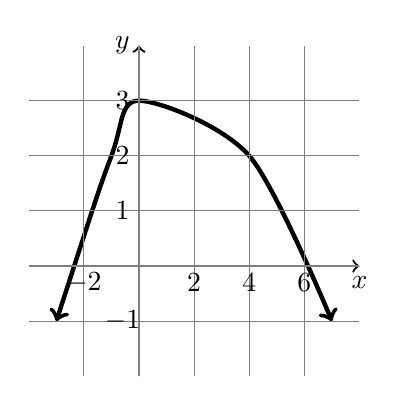
\begin{tikzpicture}[scale=.7]
\draw [ultra thick, <->] plot [smooth] coordinates {(-1.5,-1) (-.5,2) (0,3) (2,2) (3.5,-1)};
\draw[thick, ->] (-2,0) -- (4,0);\draw[thick, ->] (0,-2) -- (0,4);
\node at (4,-.3){$x$}; \node at (-.3,4){$y$};
\foreach \i in {-1,0,1,2,3}{
	\draw[gray] (-2,\i) -- (4,\i); \draw[gray] (\i,-2) -- (\i,4);
	}
\node at (-1,-.3){$-2$};\node at (1,-.3){$2$};\node at (2,-.3){$4$};\node at (3,-.3){$6$};
\node at (-.3,-1){$-1$};\node at (-.3,1){$1$};\node at (-.3,2){$2$};\node at (-.3,3){$3$};
\end{tikzpicture}
\quad \hfill \underline{\hspace{2in}}

%%WA 1.1 #11,12, 25, 27
\item For the function $f(x)=\frac{5}{x}$, find the expression $f(12+h)-f(12).$ Simplify your answer and write your answer as a single fraction.\\


\quad \hfill \underline{\hspace{2in}}
\vfill

%% Section 1.1 #42
\item Given the piecewise defined function below, determine the value(s) of $x$ such that $f(x)=-27.$

$f(x)=\begin{cases} 2x - 5 & x <0 \\ x^3 & x \geq 0 \end{cases}.$\\

\quad \hfill \underline{\hspace{2in}}
\vfill


%% factoring a quadratic
\item Solve for $x$ in the equation $x^2-2x=8.$

\quad \hfill \underline{\hspace{2in}}
\vfill

\newpage
%% Section 1.4 #19,Section 1.5 # 51,53
\item Solve for $x$ exactly in the equation $e^{2-5x}=\frac{1}{3}.$


\quad \hfill \underline{\hspace{2in}}
\vfill


%% Section 1.2 #5
\item Find all solutions to the equation $2\cos (\theta) = 1$ in the interval $[0, 2 \pi].$\\


\quad \hfill \underline{\hspace{2in}}
\vfill


%% Worksheet 1.5 + Quiz 1 Sample B
\item A table of values for the function $f(x)$ is given below. Use the table to determine $f^{-1}(5).$

\begin{tabular}{|c||c|c|c|c|c|c|c|c|c|}
$x$&-5&0&5&10&15&20&25&30&35\\
\hline
$f(x)$&40&33&18&10&-4&6&5&-2&-1/2\\
\end{tabular}

\quad \hfill \underline{\hspace{2in}}
\vspace{.2in}

%Section 1.1 # 34, Section 1.3#32,35
\item Solve the inequality $9-x^2\leq 0.$ Give your answer in interval notation.\\
\quad

\quad \hfill \underline{\hspace{2in}}
\vfill


%% Section 1.5 # 49, 50
\item Determine the domain of $f(x)=\ln(x-3).$ Give your answer in interval notation.\\
\quad

\quad \hfill \underline{\hspace{2in}}
\vfill


%%WA 1.4 #5 
 \item In the triangle below, $\sin \theta = \frac{1}{5}.$ Determine $\cos \theta.$ \hfill \underline{\hspace{2in}}\\ 
 
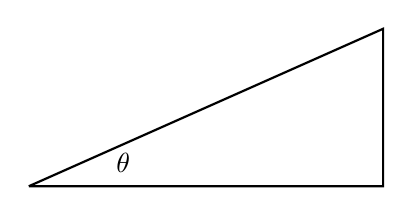
\begin{tikzpicture}
\draw[thick] (0,0)--(4.5,2) -- (4.5,0)-- (0,0);
\node at (1.2,.3){$\theta$};
\end{tikzpicture} 
\newpage
%%%%%%%%%
%Sketching Problems
%%%%%%%%%
%% Section 1.3 #1,3,5
Sketch graphs of the following functions. Label the $x$- and $y$-intercepts, if they exist. Draw in any asymptotes using dashed lines, and write the equation of the asymptote, if it exists.
%type: graph 1/x
\begin{multicols}{2}{
      % make sure you added \usepackage{enumerate}
      \vspace*{-0.45in}
%      \begin{enumerate}[(a)]

% Section 1.2 #4
  \item $f(x) =(x+1)^3$

\begin{tikzpicture}[scale=0.6][>=latex]
%x axis
\draw[->] (-5 ,0) -- (5 ,0) node[below] {$x$};
%\foreach \x in {-4,...,4}
%\draw[shift={(\x,0)}] (0pt,2pt) -- (0pt,-2pt);
%y axis
\draw[->] (0,-5) -- (0,5) node[left] {$y$};
%\foreach \y in {-4,...,4}
%\draw[shift={(0,\y)}] (2pt,0pt) -- (-2pt,0pt);
%\node[below left] at (0,0) {\footnotesize $0$};
\end{tikzpicture}
 
 
 %Section 1.4 # 12,14
 \item $f(x) = 1+e^{x} $ 

\begin{tikzpicture}[scale=0.6][>=latex]
%x axis
\draw[->] (-5 ,0) -- (5 ,0) node[below] {$x$};
%\foreach \x in {-4,...,4}
%\draw[shift={(\x,0)}] (0pt,2pt) -- (0pt,-2pt);
%y axis
\draw[->] (0,-5) -- (0,5) node[left] {$y$};
%\foreach \y in {-4,...,4}
%\draw[shift={(0,\y)}] (2pt,0pt) -- (-2pt,0pt);
\end{tikzpicture}
}
\end{multicols}

\vfill 
%\begin{multicols}{2}{
      % make sure you added \usepackage{enumerate}
      \vspace*{-0.45in}
%      \begin{enumerate}[(a)]


 \item $y =\cos(x)$ on the interval $[-2\pi, 2\pi]$

\begin{tikzpicture}[scale=0.6][>=latex]
%x axis
\draw[->] (-7 ,0) -- (7 ,0) node[below] {$x$};
%\foreach \x in {-4,...,4}
%\draw[shift={(\x,0)}] (0pt,2pt) -- (0pt,-2pt);
%y axis
\draw[->] (0,-4) -- (0,4) node[left] {$y$};
%\foreach \y in {-4,...,4}
%\draw[shift={(0,\y)}] (2pt,0pt) -- (-2pt,0pt);
%\node[below left] at (0,0) {\footnotesize $0$};
\end{tikzpicture}
 \vfill
 

\vfill


%% WA 1.3 # 11
\item Given the graph of $f(x)$ below, draw the graph of $-2f(x).$

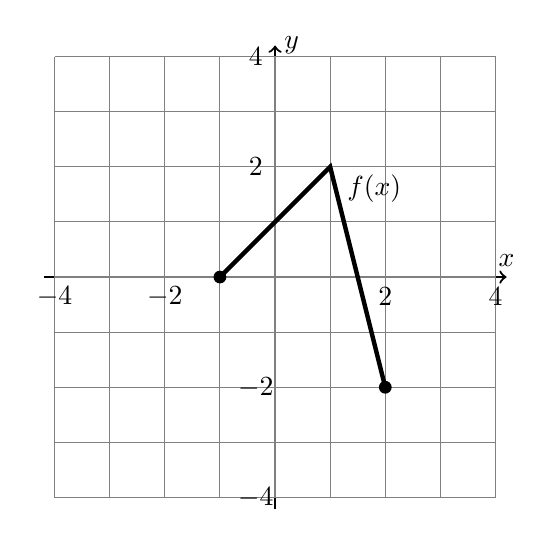
\begin{tikzpicture}[scale=.7]
\draw[thick, ->] (-4.2,0) -- (4.2,0);\draw[thick, ->] (0,-4.2) -- (0,4.2);
\node at (4.2,.3){$x$}; \node at (.3,4.2){$y$};
\foreach \i in {-4,-3,...,4}{
	\draw[gray] (-4,\i) -- (4,\i); \draw[gray] (\i,-4) -- (\i,4);

	}
\foreach \i in {-4,-2,2,4}{
	\node at (\i,-.35){$\i$};
	\node at (-.35,\i){$\i$};
	}
\node at (1.8, 1.6) {$f(x)$};
\draw[ultra thick] (-1,0) -- (1,2) -- (2,-2);	
\filldraw (-1,0) circle (3pt); \filldraw (2,-2) circle (3pt);
%\node at (-1,-.3){$-2$};\node at (1,-.3){$2$};\node at (2,-.3){$4$};\node at (3,-.3){$6$};
%\node at (-.3,-1){$-1$};\node at (-.3,1){$1$};\node at (-.3,2){$2$};\node at (-.3,3){$3$};
\end{tikzpicture}
%
\hspace{1cm}
%
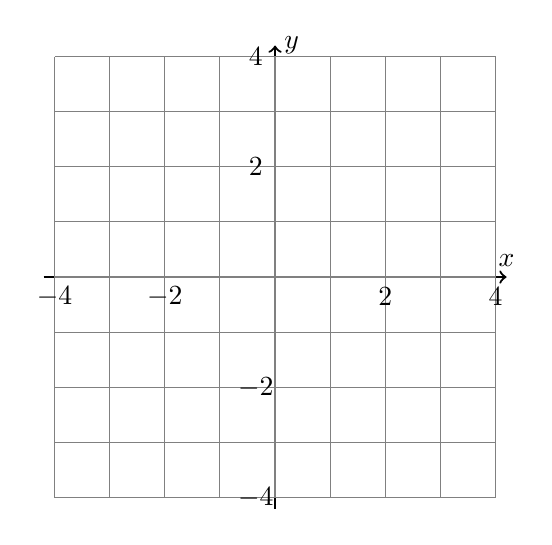
\begin{tikzpicture}[scale=.7]
\draw[thick, ->] (-4.2,0) -- (4.2,0);\draw[thick, ->] (0,-4.2) -- (0,4.2);
\node at (4.2,.3){$x$}; \node at (.3,4.2){$y$};
\foreach \i in {-4,-3,...,4}{
	\draw[gray] (-4,\i) -- (4,\i); \draw[gray] (\i,-4) -- (\i,4);

	}
\foreach \i in {-4,-2,2,4}{
	\node at (\i,-.35){$\i$};
	\node at (-.35,\i){$\i$};
	}
%\draw[ultra thick] (-1,0) -- (1,2) -- (2,-2);	
%\filldraw (-1,0) circle (3pt); \filldraw (2,-2) circle (3pt);
%\node at (-1,-.3){$-2$};\node at (1,-.3){$2$};\node at (2,-.3){$4$};\node at (3,-.3){$6$};
%\node at (-.3,-1){$-1$};\node at (-.3,1){$1$};\node at (-.3,2){$2$};\node at (-.3,3){$3$};
\end{tikzpicture}


\end{enumerate}
\end{document}
